\chapter{Appendix}

\section{From the logarithmic discretization to the Wilson's chain.\label{sec:LogarithmicDisc}}

\subsubsection{Logarithmic Discretization:}

We start with an Anderson model Hamiltonian such as the one 
in \prettyref{eq:Anderson} without magnetic field

\begin{equation}
H=\frac{U}{2}+\sum_{\sigma}\left[\left(\epsilon_{d}+\frac{U}{2}\right)d_{\sigma}^{\dagger}d_{\sigma}+\frac{U}{2}(d_{\sigma}^{\dagger}d_{\sigma}-1)^{2}+\sum_{\mathbf{k}}\ep_{\mathbf{k}}c_{\mathbf{k}\sigma}^{\dagger}c_{\mathbf{k}\sigma}+V_{\mathbf{k}}d_{\sigma}^{\dagger}c_{\mathbf{k}\sigma}+V_{\mathbf{k}}^{*}c_{\mathbf{k}\sigma}^{\dagger}d_{\sigma}\right].\label{HamWilson}
\end{equation}

At low-energies we can assume that QD couples only to s-wave states in the leads\citep{krishna-murthy_renormalization-group_1980}. This implies that that the Fermi surface is contained
in a single, isotropic conduction band extending inside some fixed cutoffs $-D$ and $D$. Thus, $\epsilon_{\mathbf{k}}$ only depends on $\left|\mathbf{k}\right|$. This makes possible to transform the sum over $\mathbf{k}$ in
equation \ref{HamWilson} into an integral over $\epsilon$ between
the energy cutoffs
\begin{eqnarray}
H & =\sum_{\sigma} & \Biggl[\left(\epsilon_{d}+\frac{U}{2}\right)d_{\sigma}^{\dagger}d_{\sigma}+\frac{U}{2}(d_{\sigma}^{\dagger}d_{\sigma}-1)^{2}+\int_{-D}^{D}\mbox{d}\epsilon\ \epsilon c_{\epsilon\sigma}^{\dagger}c_{\epsilon\sigma}\nonumber \\
 &  & \qquad\qquad\qquad\qquad\qquad\qquad+\int_{-D}^{D}\sqrt{\rho_{\sigma}(\epsilon)}\mbox{d}\epsilon\ V_{\epsilon}d_{\sigma}^{\dagger}c_{\mathbf{k}\sigma}+V_{\epsilon}^{*}c_{\epsilon\sigma}^{\dagger}d_{\sigma}\Biggr].\label{eq:hamEnergy}
\end{eqnarray}


Here $c_{\epsilon\sigma}^{\dagger}$ creates an electron with energy
$\epsilon$ and $\rho_{\sigma}(\epsilon)$ is the density of states
of the system per spin, which appears in the integral due to the change
of variable from $\mathbf{k}$ to $\epsilon\propto\left|\mathbf{k}\right|^{2}.$
Finally, we ignore the energy dependence of $\rho$ and $V_{d}$ and
we replace them by their values in the Fermi energy (This approximation
has no great relevance which is justified in \citep{krishna-murthy_renormalization-group_1980})
and we renormalize the energy band doing the replacements $k=\frac{\epsilon}{D}$
and $c_{k\sigma}:=\sqrt{D}c_{\epsilon\sigma}$ so that \prettyref{eq:hamEnergy}
becomes

\begin{eqnarray}
H & = & D\sum_{\sigma}\Biggl[\frac{1}{D}\left(\epsilon_{d}+\frac{U}{2}\right)d_{\sigma}^{\dagger}d_{\sigma}+\frac{U}{2D}(d_{\sigma}^{\dagger}d_{\sigma}-1)^{2}+\int_{-1}^{1}\mbox{d}k\ kc_{k\sigma}^{\dagger}c_{k\sigma}\nonumber \\
 &  & \qquad\qquad\qquad\qquad\qquad\qquad\qquad+\sqrt{\frac{\Gamma}{\pi D}}\int_{-1}^{1}\mbox{d}k\ d_{\sigma}^{\dagger}c_{k\sigma}+c_{k\sigma}^{\dagger}d_{\sigma}\label{eq:Norm-HamEnergy}\\
 & = & H_{d}+D\sum_{\sigma}\Biggl[\int_{-1}^{1}\mbox{d}k\ kc_{k\sigma}^{\dagger}c_{k\sigma}+\sqrt{\frac{\Gamma}{\pi D}}\int_{-1}^{1}\mbox{d}k\ d_{\sigma}^{\dagger}c_{k\sigma}+c_{k\sigma}^{\dagger}d_{\sigma}\Biggr],
\end{eqnarray}


where $\Gamma=\pi\rho V^{2}$ is associated to the lever-width \citep[(3.5)]{sindel_numerical_2005}.
At this point we have our model dependent of three unit-less constants
$\frac{\epsilon_{d}}{D}\ ,\ \frac{U}{2D}$ and $\frac{\Gamma}{\pi D}$.
The logarithmic discretization starts by defining an scaling parameter
$\Lambda\geq1$ in diving the energy domain $[-1,1]$ into an array
of intervals of the form $\{[\pm\Lambda^{-(n+1)},\pm\Lambda^{n}]\}_{n\in\mathbb{N}}$,
as we can observe in \ref{FigDiscretization}. Note that the width
of these intervals is decreasing exponentially by 
\[
d_{n}=\Lambda^{-n}\left(1-\Lambda^{-1}\right).
\]


Then inside of these energy intervals we can define a set of orthonormal
Fourier series of the form
\begin{equation}
\phi_{np}^{\pm}(\epsilon)=\begin{cases}
\frac{1}{\sqrt{d_{n}}}e^{\pm i\omega_{n}p\epsilon} & \epsilon\in[\pm\Lambda^{-(n+1)},\pm\Lambda^{n}]\\
0 & \mbox{a.o.c },
\end{cases}\label{eq:orthonormal-Fourier}
\end{equation}


with $\omega_{n}:=\frac{2\pi}{d_{n}}$ so that $\phi_{np}^{\pm}\left(\pm\Lambda^{-(n+1)}\right)=\phi_{np}^{\pm}\left(\pm\Lambda^{-n)}\right).$
Then we can decompose the creation operators $c_{k}^{\dagger}$ into
their interval-Fourier contributions as 
\begin{equation}
c_{k\sigma}^{\dagger}=\sum_{np}\phi_{np}^{+}(k)c_{np\sigma}^{+\dagger}+\phi_{np}^{-}(k)c_{np\sigma}^{-\dagger}\label{eq:Fourier-interval decomposition}
\end{equation}


with the new creation operators defined as 
\[
c_{np\sigma}^{\pm\dagger}:=\left(c_{np\sigma}^{\pm}\right)^{\dagger}=\int_{-1}^{1}\mbox{d}\epsilon\ \left[\phi_{np}^{+}(\epsilon)\right]^{*}c_{\epsilon\sigma}^{\dagger}.
\]


This decomposition \prettyref{eq:Fourier-interval decomposition}
is a simple consequence of the orthonormality of the functions defined
in \prettyref{eq:orthonormal-Fourier}. In addition we can readily
proof that $c_{np\sigma}^{\pm\dagger}$-operators satisfy the anti-commutation
relations, so that they are rightful fermionic creation operators. 

We can now use \prettyref{eq:Fourier-interval decomposition} to replace
the $k$-dependent terms in hamiltonian \prettyref{eq:Norm-HamEnergy}.
Then we obtain

\begin{eqnarray}
\int_{-1}^{1}\mbox{d}k\ c_{k\sigma}^{\dagger}d_{\sigma} & = & \int_{-1}^{1}\mbox{d}k\ \left(\sum_{np}\phi_{np}^{+}(k)c_{np\sigma}^{+\dagger}+\phi_{np}^{-}(k)c_{np\sigma}^{-\dagger}\right)d_{\sigma}\nonumber \\
 & = & \left(\sum_{np}\left(\int_{-1}^{1}\mbox{d}k\ \phi_{np}^{+}(k)\right)c_{np\sigma}^{+\dagger}+\left(\int_{-1}^{1}\mbox{d}k\ \phi_{np}^{-}(k)\right)c_{np\sigma}^{-\dagger}\right)d_{\sigma}\nonumber \\
 & = & \left(\sum_{np}\left(\int_{\Lambda^{-(n+1)}}^{\Lambda^{-n}}\mbox{d}k\ \frac{e^{i\omega_{n}pk}}{\sqrt{d_{n}}}\right)c_{np\sigma}^{+\dagger}+\left(\int_{-\Lambda^{-n}}^{-\Lambda^{-(n+1)}}\mbox{d}k\ \frac{e^{-i\omega_{n}pk}}{\sqrt{d_{n}}}\right)c_{np\sigma}^{-\dagger}\right)d_{\sigma}\nonumber \\
 & = & \left(\sum_{np}\sqrt{d_{n}}\delta_{p}c_{np\sigma}^{+\dagger}+\sqrt{d_{n}}\delta_{p}c_{np\sigma}^{-\dagger}\right)d_{\sigma}\nonumber \\
 & = & \sqrt{1-\Lambda^{-1}}\sum_{n}\Lambda^{-\frac{n}{2}}\left(c_{np\sigma}^{+\dagger}+c_{np\sigma}^{-\dagger}\right)d_{\sigma}.\label{eq:firt-Integral}
\end{eqnarray}


And 

\begin{eqnarray}
\int_{-1}^{1}\mbox{d}k\ kc_{k\sigma}^{\dagger}c_{k\sigma} & = & \sum_{n,n',p,p'}\sum_{s,s'=\pm}\left(\int_{-1}^{1}k\mbox{d}k\ \phi_{np}^{s}(k)\left(\phi_{np}^{s'}(k)\right)^{*}\right)c_{np\sigma}^{s\dagger}c_{n'p'\sigma}^{s'}\nonumber \\
 & = & \sum_{n,n',p,p'}\sum_{s,s'=\pm}\left(\frac{\delta_{nn'}\delta_{ss'}}{d_{n}}\int_{\Lambda^{-(n+1)}}^{\Lambda^{-n}}k\mbox{d}k\ e^{is\omega_{n}k\left(p-p'\right)}\right)c_{np\sigma}^{s\dagger}c_{np'\sigma}^{s}\nonumber \\
 & = & \sum_{npp'}\sum_{s=\pm}\left(\frac{s}{2}\Lambda^{-2n}\left(1-\Lambda^{-2}\right)\delta_{pp'}+\frac{1-\delta_{pp'}}{is\omega_{n}\left(p-p'\right)}\left[ke^{is\omega_{n}k\left(p-p'\right)}\right]_{\Lambda^{-(n+1)}}^{\Lambda^{-n}}\right)\frac{c_{np\sigma}^{s\dagger}c_{np'\sigma}^{s'}}{d_{n}}\nonumber \\
 & = & \frac{1}{2}\left(1+\Lambda^{-1}\right)\sum_{np}\Lambda^{-n}\left(c_{np\sigma}^{+\dagger}c_{np\sigma}^{+}-c_{np\sigma}^{-\dagger}c_{np\sigma}^{-}\right)\nonumber \\
 &  & \ \ \ \ \ \ \!\ \ \ \ \!\ \ +\sum_{n}\sum_{p\neq p'}\frac{1-\Lambda^{-1}}{2i\pi\left(p'-p\right)}\left(c_{np\sigma}^{+\dagger}c_{np'\sigma}^{+}-c_{np'\sigma}^{-\dagger}c_{np\sigma}^{-}\right)e^{\frac{2i\pi\left(p-p'\right)}{1-\Lambda^{-1}}}.\label{eq:second-integral}
\end{eqnarray}


Thus, if we replace \prettyref{eq:firt-Integral} and \prettyref{eq:second-integral}
into \prettyref{eq:Norm-HamEnergy} we will obtain a logarithmic discretization
of the hamiltonian. The next part will we to map this discretization
to an iterative process that is worth for a numerical computations. 

\subsubsection{Mapping the Anderson model to a Chain-Hamiltonian}

We are looking for a model just like the one we have in the right part of  \ref{fig:Discretization}.
This is because a Chain-Hamiltonian will give an iterative approximation
of the Anderson model with an increasing (but still controllable)
number of degrees of freedom. This will provide the rightful structure
for a numerical diagonalization of the hamiltonian. \\

To do this, observe from equations \prettyref{eq:firt-Integral},\prettyref{eq:second-integral}
that the QD ($d_{\sigma}$) couples directly only to the operators
with $p=0$$\left(c_{n0\sigma}^{\pm\dagger}\right)$. The $p\neq0$
terms will appear in the hamiltonian only because they are coupled
to $c_{np\sigma}^{+\dagger}$ in Equation \prettyref{eq:second-integral}.
Thus, as a first approximation we can neglect all terms in \prettyref{eq:second-integral}
with $p\neq0$. This leaves only the first part of \prettyref{eq:second-integral},
so that we can define $c_{n\sigma}^{\pm\dagger}:=c_{np\sigma}^{\pm\dagger}$
. Let 
\begin{equation}
f_{0\sigma}^{\dagger}=\sqrt{\frac{1-\Lambda^{-1}}{2}}\sum_{n}\Lambda^{-\frac{n}{2}}\left(c_{n\sigma}^{+\dagger}+c_{n\sigma}^{-\dagger}\right),\mbox{ so that }\sqrt{2}f_{0\sigma}^{\dagger}d_{\sigma}=\int_{-1}^{1}\mbox{d}k\ c_{k\sigma}^{\dagger}d_{\sigma}.\label{eq:f_0}
\end{equation}


Note $\left\{ f_{0\sigma}^{\dagger},f_{0\sigma}\right\} =\frac{1-\Lambda^{-1}}{2}\sum_{n}2\Lambda^{-n}=1$.
Replacing this in \prettyref{eq:Norm-HamEnergy}we get 
\[
H=H_{d}+D\sum_{\sigma}\Biggl[\sqrt{\frac{2\Gamma}{\pi D}}\left(d_{\sigma}^{\dagger}f_{0\sigma}+f_{0\sigma}^{\dagger}d_{\sigma}\right)+\frac{1}{2}\left(1+\Lambda^{-1}\right)\sum_{n}\Lambda^{-n}\left(c_{n\sigma}^{+\dagger}c_{n\sigma}^{+}-c_{n\sigma}^{-\dagger}c_{n\sigma}^{-}\right)\Biggr].
\]


$f_{0}^{\dagger}$will represent the first site of the chain-hamiltonian
in \ref{FigNRG-chain} since no other term is coupled to the dot hamiltonian.
We also have the coupling term $\xi_{0}=\sqrt{\frac{2\Gamma}{\pi D}}$.
It is possible to obtain the following $f_{m}^{\dagger}$-operators
by supposing a solution of the form 
\begin{equation}
f_{m\sigma}^{\dagger}=\sum_{n}a_{mn}^{+}c_{n\sigma}^{+\dagger}+a_{mn}^{-}c_{n\sigma}^{-\dagger}=\sum_{n}\sum_{s=\pm}a_{mn}^{s}c_{n\sigma}^{s\dagger},\label{eq:chain elements}
\end{equation}
 such that they satisfy the anti-commutation relations 
\[
\left\{ f_{m\sigma}^{\dagger},f_{m\sigma}\right\} =\delta_{mm'}\delta_{\sigma\sigma'}\ ,\ \left\{ f_{m\sigma}^{\dagger},f_{m\sigma}^{\dagger}\right\} =\left\{ f_{m\sigma}^{\dagger},f_{m\sigma}^{\dagger}\right\} =0
\]
and 
\begin{equation}
\frac{1}{2}\left(1+\Lambda^{-1}\right)\sum_{n}\Lambda^{-n}\left(c_{n\sigma}^{+\dagger}c_{n\sigma}^{+}-c_{n\sigma}^{-\dagger}c_{n\sigma}^{-}\right)=\sum_{m=0}^{\infty}\Lambda^{\frac{-m}{2}}\xi_{m}\left(f_{m\sigma}^{\dagger}f_{m+1,\sigma}+f_{m+1\sigma}^{\dagger}f_{m\sigma}\right).\label{eq:final equation}
\end{equation}


It is possible to find a solution for this system using the formula of
the right part of equation \ref{eq:final equation}. Since the relation
is only given between consecutive terms $m,m+1$ and we already have
the coefficients for $m=0$ $\left(a_{0n}^{s}=\sqrt{\frac{1-\Lambda^{-1}}{2}}\Lambda^{-\frac{n}{2}}\right).$
Then it is possible to determine the upper coefficients in a recursive way starting
from $m=0$. Supposing we can obtain the $m^{\mbox{th}}$-coefficients
$(a_{mn}^{s})$ and then finding iteratively the coefficients of $m+1\ (a_{mn}^{s})$
using the relation given by equation \prettyref{eq:final equation}.
This provides a numerical way for obtaining the $f_{m\sigma}^{\dagger}$
operators. In fact in our case, where we actually did important assumptions,
the problem can be solved analytically obtaining that the final Hamiltonian
is given by 

\begin{equation}
H=H_{d}+D\sum_{\sigma}\Biggl[\sqrt{\frac{2\Gamma}{\pi D}}\left(d_{\sigma}^{\dagger}f_{0\sigma}+f_{0\sigma}^{\dagger}d_{\sigma}\right)+\frac{1}{2}\left(1+\Lambda^{-1}\right)\sum_{n=0}^{\infty}\Lambda^{\frac{-n}{2}}\xi_{n}\left(f_{n\sigma}^{\dagger}f_{n+1,\sigma}+f_{n+1\sigma}^{\dagger}f_{n\sigma}\right)\Biggr].\label{eq:chain-Hamiltonian}
\end{equation}


with 
\[
\xi_{n}=\frac{1-\Lambda^{-n-1}}{\left(1-\Lambda^{-2n-1}\right)^{\frac{1}{2}}\left(1-\Lambda^{-2n-3}\right)^{\frac{1}{2}}}.
\]


The formal recursive-solution of this problem can be found in \citep{bulla_numerical_2008}
. Note that equation \prettyref{eq:chain-Hamiltonian} describes the
chain hamiltonian model that we where looking for in \ref{FigNRG-chain}.
Note that in the limit when $n\longrightarrow\infty$ 

\[
\Lambda^{\frac{-n}{2}}\xi_{n}\longrightarrow\frac{\Lambda^{\frac{-n}{2}}\left(1-\Lambda^{-n}\right)}{1-\Lambda^{-2n}}\sim\frac{\Lambda^{\frac{-n}{2}}}{1+\Lambda^{-n}},
\]


which implies an exponential decaying of the hopping term in the chain. 



%---------------------------------------------------------
%\section{Proof of the Graph Method for Transport Equations.\label{sec:AbsGraphmethod}}


\section{Three peak appearance in the Double Quantum Dot model.\label{sec:DoublePeak}}

The DQD model is characterized by the formation of 
a new state that entangles the two Quantum dots through the leads. This produces an anti-ferromagnetic interaction between the QDs, commonly known
as Ruderman-Kittel-Kasuya-Yosida (RKKY) interaction \citep{ruderman_indirect_1954,yosida_magnetic_1957}. As consequense, two satelite peaks will emerge in the Density of States.  




To explain this phenomenon we will take a symmetric version of Hamiltonian \eqref{General model} with $2e_i =U_i =U $ , $t_i = t$ and $t_{dots} = 0$ for $i \in \{ 1,2 \}$. 
\begin{equation}
H =\sum_{i,k,\sigma}  \frac{U_i}{2}(d_{i \sigma}^{\dagger}d_{i \sigma}-1)^{2} + t(d_{+,\dw}+d^\dagger_{+,\dw})\gamma_1 + \Gamma_i(d^\dagger_{i\sigma}c_{k\sigma}+c^\dagger_{k\sigma}d_{i\sigma}).
\label{SymModel}
\end{equation}

The symmetry of the previous Hamiltonian is suitable to apply a base change of the form 
 
\[
  d_{+ , \sigma} = \frac{1}{\sqrt{2}} (d_{1\sigma} +d_{2\sigma}) \ , \ 
  d_{- , \sigma} = \frac{1}{\sqrt{2}} (d_{1\sigma} -d_{2\sigma}).
\]


These new operators satisfy the fermionic anti-commutation relations 
 \[ \{d_{\pm , \sigma}, d^\dagger_{\pm , \sigma}\} = 1 , \{ d_{\pm , \sigma}, d^\dagger_{\mp , \sigma}\} = 0,
\]
 so that the may be considered as fermion operators. All lineal terms in \eqref{SymModel} are trivially adapted to the new base. The repulsion potential 
$$\sum_{i} (\sum_{\sigma} d_{i \sigma}^{\dagger}d_{i \sigma}-1)^{2} = (\sum_{\sigma} d_{1 \sigma}^{\dagger}d_{1 \sigma}-1)^{2} + (\sum_{\sigma} d_{2 \sigma}^{\dagger}d_{2 \sigma}-1)^{2} . $$ 
gives rise to a non-trivial interaction between the new states. To find this interaction we define the particle number operator  
\[\hat{n}_{i,\sigma}:= d^\dagger_{i,\sigma}d_{i,\sigma}.\] 

So that 
\[\hat{n}_{1,\sigma}= \frac{1}{2} \left( \hat{n}_{+,\sigma} + \hat{n}_{-,\sigma} + d^\dagger_{+,\sigma}d_{-,\sigma} + d^\dagger_{-,\sigma}d_{+,\sigma} \right) = \frac{1}{2} \left( \hat{N}_\sigma + \hat{E}_\sigma \right),  \]
with $\hat{N} = \hat{n}_{+,\sigma} + \hat{n}_{-,\sigma}$ and $\hat{E}_\sigma = d^\dagger_{+,\sigma}d_{-,\sigma} + d^\dagger_{-,\sigma}d_{+,\sigma}. $ Similarly 

\[\hat{n}_{2,\sigma}= \frac{1}{2} \left( \hat{N}_\sigma - \hat{E}_\sigma \right).  \]
Hence 

\[\sum_{i} (\sum_{\sigma} d_{i \sigma}^{\dagger}d_{i \sigma}-1)^{2} = \left(\frac{\hat{N} +\hat{E}}{2}-1 \right) ^{2} + \left( \frac{\hat{N} -\hat{E}}{2}-1 \right)^{2} = \frac{\left( \hat{N}-2 \right)^2- \hat{E}^2}{2}, \]

with $\hat{N}=\sum_\sigma \hat{N}_\sigma $ , $\hat{E}=\sum_\sigma \hat{E}_\sigma $. Note that opeator $\hat{N}$ represents the total occupation number inside both dots. If this occupation is different than $2$ there is an imbalance between particles and dots that is punished by this term. The term $E^2$ is much more interesting since this one is the responsible for the emergence of satellite peaks in the DOS. To understand what it makes it is simple to observe its results when applied to a based ordered by $\vert + , - \rangle$. 
\[ \hat{E}^2 \vert \up , 0 \rangle =  \hat{E} \vert 0 , \up \rangle = \vert \up , 0 \rangle   \] 
\[ \hat{E}^2 \vert \up , \dw \rangle =  \hat{E} \left( \vert 0 , \up\!\dw \rangle + \vert \up\!\dw , 0 \rangle \right) = 2\vert \up , \dw \rangle - 2\vert \dw , \up \rangle  \]





The new Hamiltonian 
\begin{equation}
H = \sum_{\sigma}  \frac{U}{4}\left( \left( \hat{N}-2 \right)^2- \hat{E}^2 \right) + \frac{t}{\sqrt{2}} (d_{+,\dw}+d^\dagger_{+,\dw})\gamma_1 
 +  \frac{\Gamma}{\sqrt{2}}\sum_{ k}(d^\dagger_{+,\sigma}c_{k\sigma}+c^\dagger_{k\sigma}d_{+,\sigma})
\label{t+}
\end{equation}
is represented in \ref{fig:ExchangeMod}

% \begin{figure*}[h]
% \centering
% 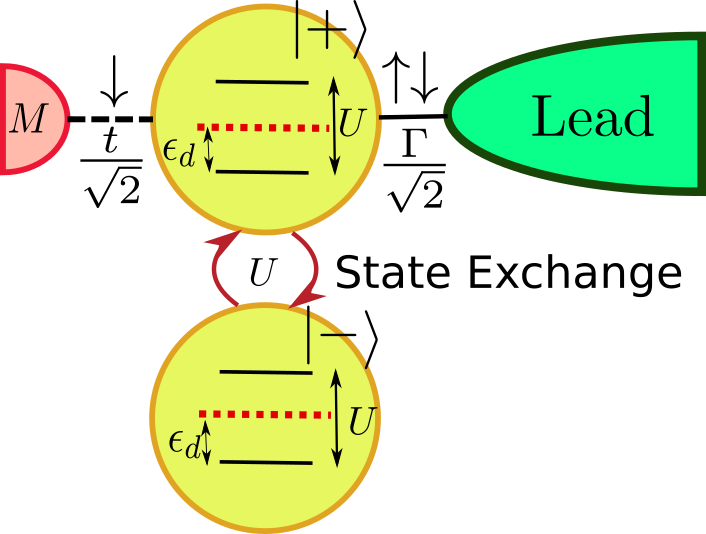
\includegraphics[scale=0.4]{IMAGES/ExchangeMod.png}
% \caption{\label{fig:ExchangeMod} General model.} 
% \end{figure*}




%\begin{equation}
%H = \sum_{i,k} \left(\epsilon_{d}+\frac{U}{2}\right)d_{\sigma}^{\dagger}d_{\sigma}+\frac{U_i}{2}(d_{\sigma}^{\dagger}d_{\sigma}-1)^{2} + t_i d_i+d^\dagger_i \gamma_1 + \Gamma_i(d_{\sigma}c_{\sigma})
%\end{equation}


We can explain this three-peak as the result of a new strong coupling interaction characterized by the spin exchange between both dots. 
%HERE COMES THE CHANGE OF BASIS 

In addition, the spin-up DOS at the Fermi energy grows faster than the spin-down DOS, breaking the initial spin-symmetry when $t_1=t_2=0$. At $t_1=t_2=0.02D$ the spin-up DOS at the fermi energy doubles the spin-down DOS which implies that the Majorana signature  is present in both dots. %I need to write what is this Majorana signature about. 
Indeed \ref{fig:MSig/Shift_t1=t2} shows that the relation $\frac{\rho_\up(0)}{\rho_\up(0)}$ increases continuously from $1$ to $2$. Note that the Majorana is completely attached when the coupling $t_1$ reaches the order of $0.01D$ .

\section{Initial DQD-Majorana Hamiltonian.\label{sec:Double-Dot-Majorana-Hamiltonian.}}

$H_{N_{\uparrow}=0,P_{\downarrow}=-1}:$
\[
\begin{array}{c}
\vert\downarrow,\downarrow,\downarrow\rangle\rightarrow\\
\vert0,0,\downarrow\rangle\rightarrow\\
\vert0,\downarrow,0\rangle\rightarrow\\
\vert\downarrow,0,0\rangle\rightarrow
\end{array}\left[\begin{array}{cccc}
\epsilon_{d}^{+}+\frac{U^{+}}{2}-2h+\epsilon_{m} & 0 & -\tilde{t}_{+1} & \tilde{t}_{+2}\\
0 & \frac{U^{+}}{2}+\epsilon_{m} & \tilde{t}_{-2}^{*} & \tilde{t}_{-1}^{*}\\
-\tilde{t}_{+1}^{*} & \tilde{t}_{-2} & \epsilon_{d_{2}}+\frac{U^{+}}{2}-h-\epsilon_{m} & t\\
\tilde{t}_{+2}^{*} & \tilde{t}_{-1} & t^{*} & \epsilon_{d_{1}}+\frac{U^{+}}{2}-h-\epsilon_{m}
\end{array}\right]
\]


$H_{N_{\uparrow}=0,P_{\downarrow}=1}:$
\[
\begin{array}{c}
\vert0,0,0\rangle\rightarrow\\
\vert\downarrow,\downarrow,0\rangle\rightarrow\\
\vert\downarrow,0,\downarrow\rangle\rightarrow\\
\vert0,\downarrow,\downarrow\rangle\rightarrow
\end{array}\left[\begin{array}{cccc}
\frac{U^{+}}{2}-\epsilon_{m} & 0 & \tilde{t}_{+1} & \tilde{t}_{+2}\\
0 & \epsilon_{d}^{+}+\frac{U^{+}}{2}-2h-\epsilon_{m} & \tilde{t}_{-2}^{*} & -\tilde{t}_{-1}^{*}\\
\tilde{t}_{+1}^{*} & \tilde{t}_{-2} & \epsilon_{d_{1}}+\frac{U^{+}}{2}-h+\epsilon_{m} & t\\
\tilde{t}_{+2}^{*} & -\tilde{t}_{-1} & t^{*} & \epsilon_{d_{2}}+\frac{U^{+}}{2}-h+\epsilon_{m}
\end{array}\right]
\]


$H_{N_{\uparrow}=2,P_{\downarrow}=-1}:$
\[
\begin{array}{c}
\vert\uparrow\!\downarrow,\uparrow\!\downarrow,\downarrow\rangle\rightarrow\\
\vert\uparrow,\uparrow,\downarrow\rangle\rightarrow\\
\vert\uparrow,\uparrow\!\downarrow,0\rangle\rightarrow\\
\vert\uparrow\!\downarrow,\uparrow,0\rangle\rightarrow
\end{array}\left[\begin{array}{cccc}
2\epsilon_{d}^{+}+\frac{3U^{+}}{2}+\epsilon_{m} & 0 & \tilde{t}_{+1} & \tilde{t}_{+2}\\
0 & \epsilon_{d}^{+}+\frac{U^{+}}{2}+2h+\epsilon_{m} & \tilde{t}_{-2}^{*} & -\tilde{t}_{-1}^{*}\\
\tilde{t}_{+1}^{*} & \tilde{t}_{-2} & f(d_{1},d_{2})+h-\epsilon_{m} & -t\\
\tilde{t}_{+2}^{*} & -\tilde{t}_{-1} & -t^{*} & f(d_{2},d_{1})+h-\epsilon_{m}
\end{array}\right]
\]


with $f(d_{i},d_{j})=\epsilon_{d_{i}}+\frac{U_{i}}{2}+2\epsilon_{d_{j}}+\frac{3U_{j}}{2}.$

$H_{N_{\uparrow}=2,P_{\downarrow}=1}:$
\[
\begin{array}{c}
\vert\uparrow,\uparrow,0\rangle\rightarrow\\
\vert\uparrow\!\downarrow,\uparrow\!\downarrow,0\rangle\rightarrow\\
\vert\uparrow\!\downarrow,\uparrow,\downarrow\rangle\rightarrow\\
\vert\uparrow,\uparrow\!\downarrow,\downarrow\rangle\rightarrow
\end{array}\left[\begin{array}{cccc}
\epsilon_{d}^{+}+\frac{U^{+}}{2}+2h-\epsilon_{m} & 0 & -\tilde{t}_{+1} & \tilde{t}_{+2}\\
0 & 2\epsilon_{d}^{+}+\frac{3U^{+}}{2}-\epsilon_{m} & \tilde{t}_{-2}^{*} & \tilde{t}_{-1}^{*}\\
-\tilde{t}_{+1}^{*} & \tilde{t}_{-2} & f(d_{2},d_{1})+h+\epsilon_{m} & -t\\
\tilde{t}_{+2}^{*} & \tilde{t}_{-1} & -t^{*} & f(d_{1},d_{2})+h+\epsilon_{m}
\end{array}\right]
\]
